\chapter{Abbildungen}\label{appen}
\begin{figure}[ht]
    \centering
    \begin{subfigure}{0.45\textwidth}
        \centering
        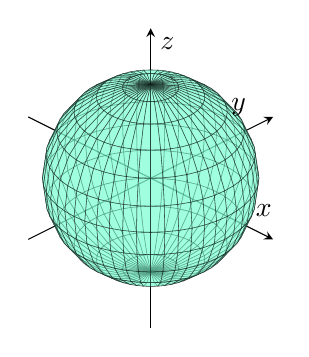
\begin{tikzpicture}
    \begin{axis}[%
        axis equal,
        width=8.5cm,
        height=8.5cm,
        colormap/blackwhite,
        axis lines = center,
        xlabel = {$x$},
        ylabel = {$y$},
        zlabel = {$z$},
        ticks=none, 
        enlargelimits=0.3,
        view/h=45,
        scale uniformly strategy=units only,
    ]
    \addplot3[%
        opacity = 0.5,
        surf,
        line width=0.2pt,
        fill=Aquamarine,
        point meta=100,
        z buffer = sort,
        samples = 25,
        variable = \u,
        variable y = \v,
        domain = 0:180,
        y domain = 0:360,
    ]
    ({cos(u)*sin(v)}, {sin(u)*sin(v)}, {cos(v)});
    \end{axis}
\end{tikzpicture}
    \end{subfigure}
    \begin{subfigure}{0.45\textwidth}
        \centering
        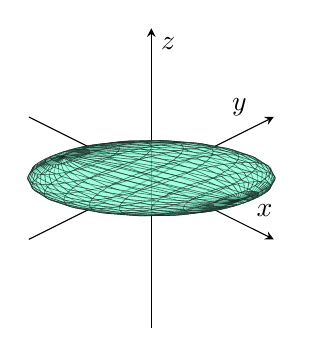
\begin{tikzpicture}
    \begin{axis}[%
        axis equal,
        width=8.5cm,
        height=8.5cm,
        colormap/blackwhite,
        axis lines = center,
        xlabel = {$x$},
        ylabel = {$y$},
        zlabel = {$z$},
        ticks=none, 
        enlargelimits=0.3,
        view/h=45,
        scale uniformly strategy=units only,
        zmin=-0.1,
        zmax=0.1,
        xmin=-3.5,
        xmax=3.5,
        ymin=-3.5,
        ymax=3.5,
        zmin=-3.5, 
        zmax=3.5
    ]
    \addplot3[%
        opacity = 0.5,
        surf,
        line width=0.2pt,
        fill=Aquamarine,
        point meta=100,
        z buffer = sort,
        samples = 25,
        variable = \u,
        variable y = \v,
        domain = 0:180,
        y domain = 0:360,
    ]
    (
        {4/2*cos(u)*sin(v) + 4/2*cos(v) -cos(u)*sin(v) - sin(u)*sin(v) + cos(v) }, 
        {4/2*cos(u)*sin(v) + 4/2*cos(v) +cos(u)*sin(v) +sin(u)*sin(v) -cos(v)}, 
        {0} 
    );
    \end{axis}
\end{tikzpicture}
    \end{subfigure}
    \caption{Wirkung von \(A\) auf die Einheitssphäre}\label{fig:sph}
\end{figure}

\begin{figure}[ht]
    \centering
    \begin{tikzpicture}
        \begin{axis}[
            axis lines = middle,
            xlabel = {Horror},
            ylabel = {Drama},
            xmin = -2, xmax = 2,
            ymin = -2, ymax = 2,
            xtick=\empty,
            ytick=\empty,
            legend pos = north west,
            legend cell align=left,
        ]

        \addplot[only marks, mark=o, mark size=2.5, blue] coordinates {
            (-1,0.1) (0,0.5) (1,0.6) (-0.5,-1) (0.86,-0.2) (-0.1,1)
        };
        \addlegendentry{Nutzer}

        \addplot[only marks, mark=x, mark size=2.5, red] coordinates {
            (-1,-0.5) (0.5,0.4) (1,-1) (0,-1.5)
        };
        \addlegendentry{Filme}

        \end{axis}
    \end{tikzpicture}
    \caption{Gemeinsamer latenter Raum von Nutzern und Filmen}\label{fig:app:lat}
\end{figure}

\begin{figure}[!t]
    \centering
    \resizebox{0.85\textwidth}{!}{ 
    \begin{minipage}{\textwidth}
    \captionsetup[subfigure]{justification=centering}
    \begin{subfigure}{\textwidth}
        \centering
        \caption{\(n=2\)}
        \begin{tabular}{lrrrrr}
    \toprule
    & \multicolumn{2}{c}{Merkmale} \\
    \cmidrule(lr){2-3}
    Weine & A & B \\ 
    \midrule
    Wein 1  & 1,3 & -0,4  \\
    Wein 2 & -1,6 & 2,1 \\
    Wein 3 & 1,2 & 0,7 \\
    Wein 4 & -2,1 & 0,6 \\
    Wein 5 & 0,8 & 0,6 \\
    Wein 6 & -0,3 & 1,6 \\
    \bottomrule
\end{tabular}
        \hspace{35pt}
        \begin{tikzpicture}[baseline=(current bounding box.center)]
    \begin{axis}[
        xlabel={\(A\)},
        ylabel={\(B\)},
        width=0.45\textwidth,
        anchor=center,
    ]
    \addplot[only marks,mark options={fill=black, color=black}] coordinates {
        (1.3,-0.4) 
        (-1.6,2.1)
        (1.2,0.7)
        (-2.1,0.6)
        (0.8,0.6)
        (-0.3,1.6)
    };
    \end{axis}
\end{tikzpicture}
    \end{subfigure}
    \begin{subfigure}{\textwidth}
        \centering
        \caption{\(n=3\)}
        \begin{tabular}{lrrrrr}
    \toprule
    & \multicolumn{3}{c}{Merkmale} \\
    \cmidrule(lr){2-4}
    Weine & A & B & C \\ 
    \midrule
    Wein 1  & 1,3 & -0,4 & 1,9 \\
    Wein 2 & -1,6 & 2,1 & 0,2 \\
    Wein 3 & 1,2 & 0,7 & 0,4 \\
    Wein 4 & -2,1 & 0,6 & -0,2 \\
    Wein 5 & 0,8 & 0,6 & 1,1 \\
    Wein 6 & -0,3 & 1,6 & 0.8 \\
    \bottomrule
\end{tabular}
        \hspace{17pt}
        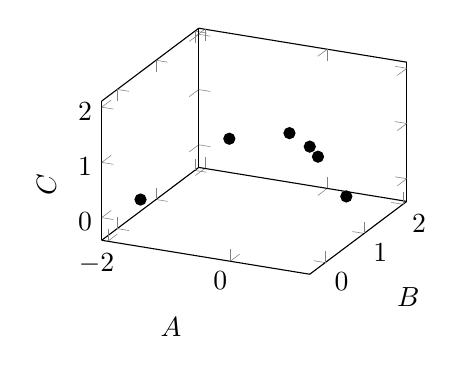
\begin{tikzpicture}[baseline=(current bounding box.center)]
    \begin{axis}[
        xlabel={\(A\)},
        ylabel={\(B\)},
        zlabel={\(C\)},
        width=0.45\textwidth,
        anchor=center,
    ]
    \addplot3+[only marks,mark options={fill=black, color=black}] coordinates {
        (1.3,-0.4,1.9) 
        (-1.6,2.1,0.2)
        (1.2,0.7,0.4)
        (-2.1,0.6,-0.2)
        (0.8,0.6,1.1)
        (-0.3,1.6,0.8)
    };
    \end{axis}
\end{tikzpicture}
    \end{subfigure}
    \begin{subfigure}{\textwidth}
        \caption{\(n=4\)}
        \begin{tabular}{lrrrrrr}
    \toprule
    & \multicolumn{4}{c}{Merkmale} \\
    \cmidrule(lr){2-5}
    Wein & A & B & C & D \\ 
    \midrule
    Wein 1 & 1,3 & -0,4 & 1,9 & 0.7 \\
    Wein 2 & -1,6 & 2,1 & 0,2 & 0.9 \\
    Wein 3 & 1,2 & 0,7 & 0,4 & 1.3 \\
    Wein 4 & -2,1 & 0,6 & -0,2 & 0.5 \\
    Wein 5 & 0,8 & 0,6 & 1,1 & -0.8 \\
    Wein 6 & -0,3 & 1,6 & 0.8 & -1.3 \\
    \bottomrule
\end{tabular}
        \hspace{45pt}
        
\begin{tikzpicture}[baseline=(current bounding box.center)]
    \draw[thick] (-2,-2) rectangle (2,2);
    \node at (0,0) {\Huge \textbf{?}};
\end{tikzpicture}
    \end{subfigure}
    \end{minipage}
    }
    \caption{Darstellung von Daten in verschiedenen Dimensionen}\label{fig:pcadim}
\end{figure}